% ==================================================================
% BAS vs. Horseshoe --- includable section fragment
% Meant to be \input{} / \include{} inside a larger document.
%
% Parent preamble must load: amsmath, amssymb, graphicx, booktabs,
%   siunitx  (and set \sisetup{table-format=1.3,round-mode=places,
%   round-precision=3} or equivalent).
% Figures fig1.png / fig2.png must sit where \graphicspath can find them.
% ==================================================================

\section{Feature selection cross-check with BAS}
\noindent
After fitting our feature-selection model based on a horseshoe prior, we
would like to compare it with a Bayesian Adaptive Sampling (BAS) model in
order to verify whether the two methods agree on which covariates are more
useful in explaining the target variable.

With $23$ predictors, $2^{23}\approx 8.4$ million candidate models are far
too many to enumerate exhaustively, so we use \texttt{method = "MCMC"} in
BAS to stochastically search the model space. A later section assesses
whether this search suffers from instability or not.

Table~\ref{tab:bas-top} reports the marginal posterior inclusion
probabilities $P(\beta_j \neq 0 \mid Y)$ for every predictor, together with
the five highest-probability models returned by the search and their
summary statistics (Bayes factor, posterior probability, $R^2$,
dimension and log marginal likelihood).

\begin{table}[htbp]
\centering
\footnotesize
\caption{Marginal posterior inclusion probabilities and the top five
models identified by the BAS MCMC search. A value of $1.000$/$0.000$ in a
model column indicates the predictor is included/excluded in that model.}
\label{tab:bas-top}
\begin{tabular}{l S S S S S S}
\toprule
& {$P(\beta\!\neq\!0\mid Y)$} & {Model 1} & {Model 2} & {Model 3} & {Model 4} & {Model 5}\\
\midrule
Intercept            & 1.000 & 1.000 & 1.000 & 1.000 & 1.000 & 1.000\\
seat\_comfort        & 0.803 & 1.000 & 1.000 & 1.000 & 1.000 & 0.000\\
time\_convenient     & 0.973 & 1.000 & 1.000 & 1.000 & 1.000 & 1.000\\
food\_drink          & 0.500 & 1.000 & 0.000 & 1.000 & 0.000 & 0.000\\
gate\_location       & 0.037 & 0.000 & 0.000 & 0.000 & 0.000 & 0.000\\
wifi                 & 0.049 & 0.000 & 0.000 & 0.000 & 0.000 & 0.000\\
entertainment        & 1.000 & 1.000 & 1.000 & 1.000 & 1.000 & 1.000\\
online\_support      & 0.220 & 0.000 & 0.000 & 0.000 & 0.000 & 0.000\\
ease\_booking        & 0.954 & 1.000 & 1.000 & 1.000 & 1.000 & 1.000\\
onboard\_service     & 0.996 & 1.000 & 1.000 & 1.000 & 1.000 & 1.000\\
legroom              & 0.965 & 1.000 & 1.000 & 1.000 & 1.000 & 1.000\\
baggage              & 0.073 & 0.000 & 0.000 & 0.000 & 0.000 & 0.000\\
checkin              & 0.986 & 1.000 & 1.000 & 1.000 & 1.000 & 1.000\\
cleanliness          & 0.310 & 0.000 & 0.000 & 0.000 & 0.000 & 0.000\\
online\_boarding     & 0.029 & 0.000 & 0.000 & 0.000 & 0.000 & 0.000\\
Age\_std             & 0.037 & 0.000 & 0.000 & 0.000 & 0.000 & 0.000\\
FlightDist\_std      & 0.035 & 0.000 & 0.000 & 0.000 & 0.000 & 0.000\\
Class\_EcoPlus       & 0.029 & 0.000 & 0.000 & 0.000 & 0.000 & 0.000\\
Class\_Business      & 0.993 & 1.000 & 1.000 & 1.000 & 1.000 & 1.000\\
logdep\_std          & 0.092 & 0.000 & 0.000 & 0.000 & 0.000 & 0.000\\
TypeTravel\_Personal & 0.451 & 0.000 & 0.000 & 1.000 & 1.000 & 1.000\\
CustType\_disloyal   & 1.000 & 1.000 & 1.000 & 1.000 & 1.000 & 1.000\\
logmid\_delay        & 0.031 & 0.000 & 0.000 & 0.000 & 0.000 & 0.000\\
\midrule
BF        & {NA} & 1.000    & 0.574    & 0.477    & 0.369    & 0.268\\
PostProbs & {NA} & 0.128    & 0.071    & 0.059    & 0.048    & 0.033\\
$R^2$     & {NA} & 0.426    & 0.421    & 0.430    & 0.425    & 0.420\\
dim       & {NA} & 11.000   & 10.000   & 12.000   & 11.000   & 10.000\\
logmarg   & {NA} & -516.838 & -517.392 & -517.578 & -517.835 & -518.155\\
\bottomrule
\end{tabular}
\end{table}

% ==================================================================
\section{Parameter-space convergence}


% ==================================================================
We now test the goodness of the MCMC search over the parameter space
executed by BAS.

% ------------------------------------------------------------------
\subsection*{Convergence within one run}
% ------------------------------------------------------------------
BAS reports two independent estimates of each posterior inclusion
probability:
\begin{itemize}
  \item \texttt{probne0.RB}: takes the set of distinct visited models that
  contain variable $j$, uses their marginal likelihoods, renormalises and
  sums the mass of those models;
  \item \texttt{probne0.MCMC}: the raw fraction of iterations the chain
  spent in some model containing variable $j$.
\end{itemize}
If the chain has converged, the two estimates should agree closely.

The correlation between the two estimates is $0.9999$ and the maximum
absolute difference is $0.014$: the points sit essentially on the diagonal
(Figure~\ref{fig:conv}), the sign that this run has converged.

\begin{figure}[htbp]
\centering
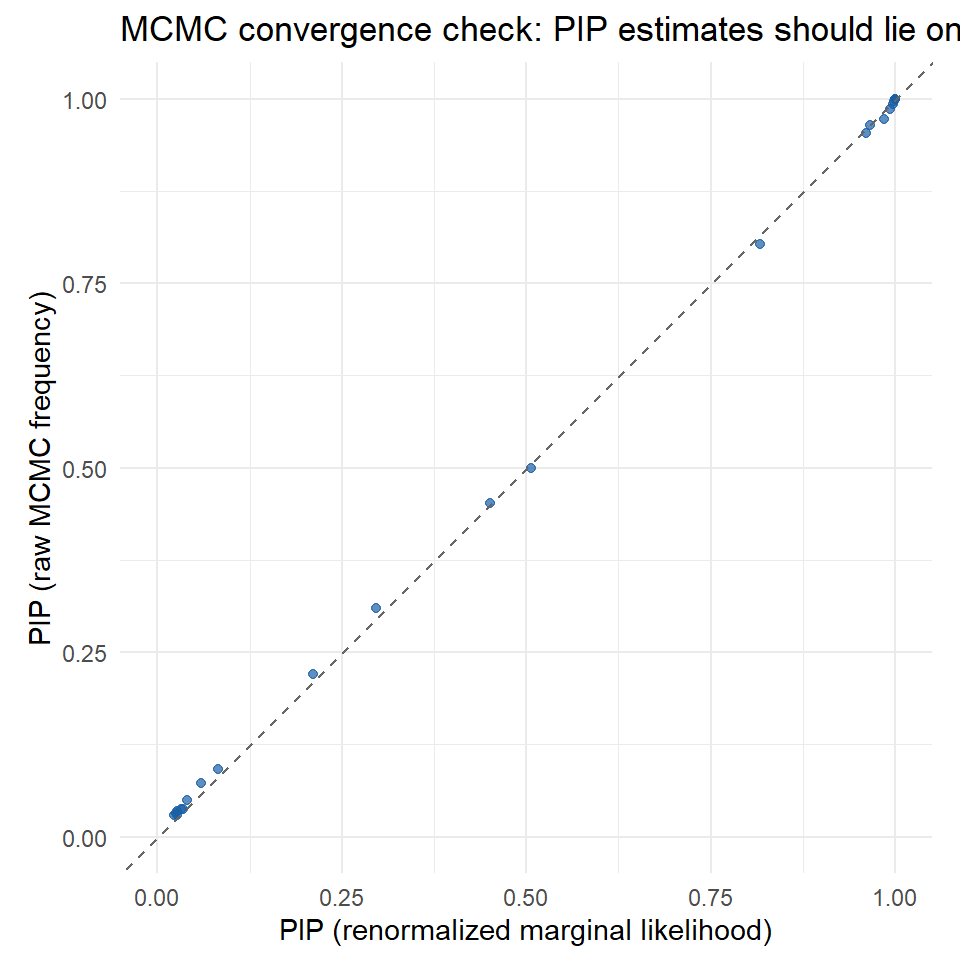
\includegraphics[width=0.6\textwidth]{img/bas_crosscheck/BAS_PIP_comparison.png}
\caption{MCMC convergence check. Renormalised-marginal-likelihood
inclusion probabilities (x-axis) against raw MCMC-frequency inclusion
probabilities (y-axis); points lying on the dashed diagonal indicate the
two estimates agree.}
\label{fig:conv}
\end{figure}

% ------------------------------------------------------------------
\subsection*{Stability across seeds}
% ------------------------------------------------------------------
We refit the identical model twice more with different random seeds and
compare the posterior inclusion probabilities (PIPs) to check whether they
agree. Table~\ref{tab:seeds} lists the predictors with the largest spread,
ordered by the range across the three seeds.

\begin{table}[htbp]
\centering
\caption{Posterior inclusion probabilities across three random seeds, with
the range (max $-$ min) per predictor. Only the eight most variable
predictors are shown.}
\label{tab:seeds}
\begin{tabular}{l S S S S}
\toprule
term & {seed123} & {seed1} & {seed2} & {range}\\
\midrule
seat\_comfort        & 0.803 & 0.841 & 0.826 & 0.038\\
food\_drink          & 0.500 & 0.533 & 0.511 & 0.033\\
online\_support      & 0.220 & 0.228 & 0.204 & 0.024\\
cleanliness          & 0.310 & 0.297 & 0.316 & 0.019\\
TypeTravel\_Personal & 0.451 & 0.439 & 0.457 & 0.017\\
legroom              & 0.965 & 0.951 & 0.959 & 0.013\\
time\_convenient     & 0.973 & 0.979 & 0.983 & 0.011\\
baggage              & 0.073 & 0.065 & 0.064 & 0.009\\
\bottomrule
\end{tabular}
\end{table}

% ------------------------------------------------------------------
\subsection*{BIC prior as a robustness check}
% ------------------------------------------------------------------
We try another prior on the $\beta$ coefficients: if the search is stable,
the effect of the prior should vanish once the number of iterations is
large enough. Table~\ref{tab:bic} compares the $g$-prior PIPs with those
obtained under a BIC-based prior.

\begin{table}[htbp]
\centering
\caption{Posterior inclusion probabilities under the $g$-prior and the
BIC-based prior, with the absolute difference per predictor (six most
affected predictors shown).}
\label{tab:bic}
\begin{tabular}{l S S S}
\toprule
term & {g\_prior} & {BIC} & {abs\_diff}\\
\midrule
online\_support & 0.220 & 0.224 & 0.004\\
cleanliness     & 0.310 & 0.314 & 0.004\\
seat\_comfort   & 0.803 & 0.801 & 0.002\\
food\_drink     & 0.500 & 0.498 & 0.002\\
ease\_booking   & 0.954 & 0.952 & 0.002\\
legroom         & 0.965 & 0.967 & 0.002\\
\bottomrule
\end{tabular}
\end{table}

With $100{,}000$ MCMC iterations, PIPs move by at most $0.038$ across the
three seeds and by at most $0.004$ between the $g$-prior and the BIC-based
prior. Given the number of MCMC iterations, the search proves itself to be
stable.

% ==================================================================
\section{BAS vs.\ Horseshoe: model comparison}
\label{app:bas_vs_hs}

% ==================================================================
Finally, we compare the models selected by the two approaches and check on
which coefficients they agree and on which they do not. Figure~\ref{fig:cmp}
plots each predictor's BAS inclusion probability against the horseshoe's
$1-\kappa_j$ shrinkage measure, colouring predictors by whether the two
methods make the same signal/noise call.

\begin{figure}[htbp]
\centering
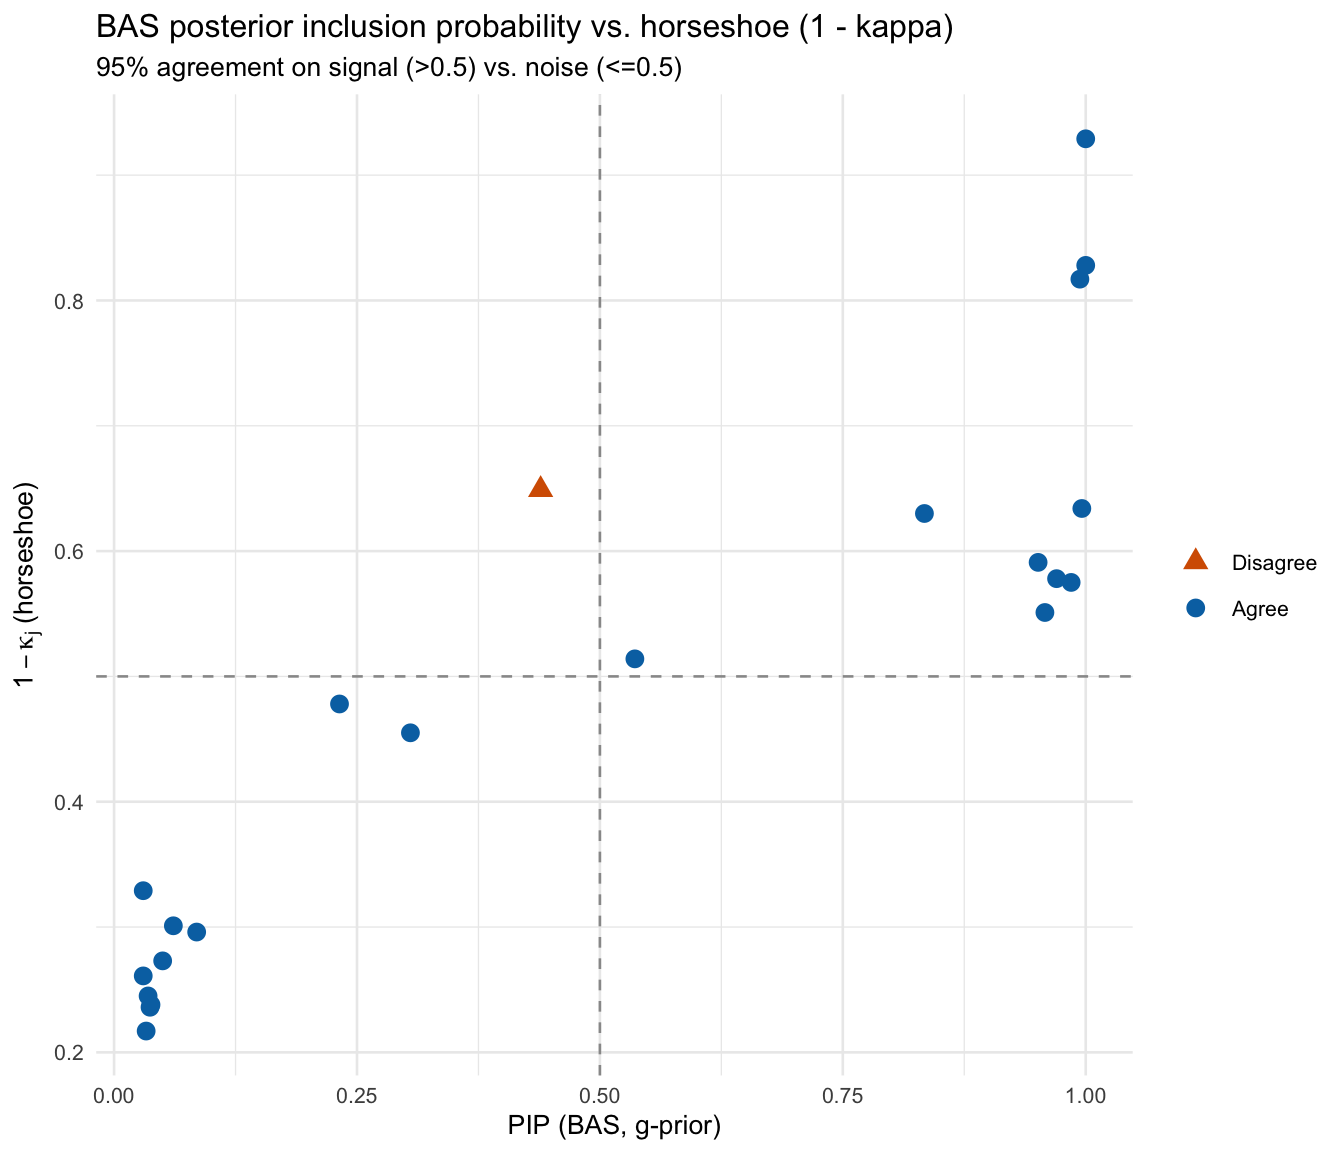
\includegraphics[width=0.75\textwidth]{img/bas_crosscheck/bas_vs_horseshoe_comparison.png}
\caption{BAS posterior inclusion probability (x-axis) against the
horseshoe's $1-\kappa_j$ (y-axis). Dashed lines mark the $0.5$ signal/noise
cutoff for each method; green points denote agreement, the red point
denotes the single disagreement.}
\label{fig:cmp}
\end{figure}

91\% of the 22 predictors get the same signal/noise call from BAS's
model-space search and from the horseshoe's continuous shrinkage --
two structurally different estimation strategies (discrete model
averaging vs.\ a single shrinkage prior) landing on the same handful
of variables. The two disagreements are genuine borderline cases in
both methods: \texttt{Personal Travel} (PIP 0.439, $\kappa = 0.353$)
sits just on opposite sides of each method's 0.5 cutoff, and
\texttt{Food and drink} (PIP $\approx 0.50$, $\kappa = 0.489$) sits
essentially on the cutoff for both methods and flips across MCMC
seeds (Table~18) -- not a real contradiction between the two
approaches, but two variables where the signal is genuinely too weak
to classify with confidence.